\documentclass[11pt,a4paper]{article}
\usepackage{geometry}
\geometry{top=2.5cm, bottom=2.5cm, left=2.5cm, right=2.5cm}
\usepackage{graphicx}
\usepackage{adjustbox}
\usepackage{setspace}
\usepackage{tikz}
\usetikzlibrary{calc}
\usepackage{eso-pic}
\usepackage{titlesec}
\usepackage{float}
\usepackage{array}
\usepackage{booktabs}
\usepackage{xcolor}
\usepackage{caption}

\usepackage{listings}
\captionsetup[lstlisting]{labelformat=empty}
\lstset{
    language=Verilog,
    basicstyle=\ttfamily\footnotesize,
    keywordstyle=\color{blue}\bfseries,
    identifierstyle=\color{black},
    stringstyle=\color{purple},
    commentstyle=\color{green},
    showstringspaces=false,
    numbers=left,
    numberstyle=\tiny\color{gray},
    frame=single,
    rulecolor=\color{black!30},
    breaklines=true,
    backgroundcolor=\color{gray!5},
    captionpos=b
}

\titleformat{\section}{\fontsize{18pt}{22pt}\bfseries}{\thesection}{1em}{}
\titleformat{\subsection}{\fontsize{15pt}{19pt}\bfseries}{\thesubsection}{1em}{}
\titleformat{\subsubsection}{\fontsize{13pt}{17pt}\bfseries}{\thesubsubsection}{1em}{}

\usepackage{tocloft}
\renewcommand{\cftsecleader}{\cftdotfill{\cftdotsep}}

\usepackage{xepersian}
\settextfont{XB Niloofar}
\setdigitfont{XB Niloofar}

\begin{document}

\AddToShipoutPictureBG{
    \begin{tikzpicture}[remember picture, overlay]
        \node[draw, line width=2.5pt, minimum width=\paperwidth-2cm, minimum height=\paperheight-2cm, inner sep=0pt] at (current page.center) {};
        \node[draw, line width=1.0pt, minimum width=\paperwidth-2.3cm, minimum height=\paperheight-2.3cm, inner sep=0pt] at (current page.center) {};
    \end{tikzpicture}
}

\begin{titlepage}
    \centering
    \vspace*{0.2cm}
    
\includegraphics[width=3.5cm]{images/logo.png} \\[0.4cm] 
    {\fontsize{14pt}{18pt}\selectfont دانشگاه صنعتی شریف} \\[0.2cm]
    {\fontsize{14pt}{18pt}\selectfont دانشکده مهندسی کامپیوتر} \\[0.6cm]
    {\fontsize{18pt}{22pt}\bfseries گزارش کار آزمایش هشتم}

    \vspace{1.2cm}
    {\fontsize{12pt}{16pt}\selectfont عنوان:} \\[0.3cm]
    {\fontsize{22pt}{28pt}\bfseries طراحی واحد محاسبه و منطق مختلط} \\[0.3cm]
    
    \vspace{1.0cm}
    {\fontsize{12pt}{16pt}\selectfont نام درس:} \\[0.3cm]
    {\fontsize{14pt}{18pt}\bfseries آزمایشگاه طراحی سامانه‌های رقمی}

    \vspace{1.0cm}
    {\fontsize{12pt}{16pt}\selectfont تابستان ۱۴۰۵}

    \vspace{1.0cm}
    {\fontsize{12pt}{16pt}\selectfont استاد:} \\[0.3cm]
    {\fontsize{14pt}{18pt}\bfseries دکتر اجلالی}
    
    \vspace{0.6cm}
    {\fontsize{12pt}{16pt}\selectfont دستیار استاد:} \\[0.3cm]
    {\fontsize{14pt}{18pt}\bfseries علی اثنی عشری}

\vspace{1.0cm}
{\fontsize{12pt}{16pt}\selectfont گروه ۲\par}
\vspace{0.3cm}
{\fontsize{14pt}{20pt}\bfseries
علی سلطانی - 403106092\\[0.15cm]
یگانه کربلایی - 403106527\\[0.15cm]
محمدمهدی مرادی - 403106681\par}

    \vfill
\end{titlepage}

\newpage
\tableofcontents
\newpage

\section{هدف و صورت آزمایش}
هدف از این آزمایش، طراحی، توصیف سخت‌افزاری و پیاده‌سازی یک واحد منطق حسابی برای اعداد مختلط است. طراحی باید به صورت پیمانه‌ای\LTRfootnote{Modular} انجام شود؛ به این معنا که هر بخش محاسباتی به صورت یک پیمانه مستقل طراحی شده و سپس با اتصال این پیمانه‌ها به یکدیگر یک ساختار کامل‌تر ساخته شود. در نهایت این واحد باید بتواند دستورهای مختلف محاسباتی مربوط به اعداد مختلط را از یک حافظه ۳۲ کلمه‌ای دریافت کرده و آن‌ها را اجرا کند.

\subsection{چالش ساختاری و راهبرد طراحی}
یکی از چالش‌های اصلی و ظریف این آزمایش، وجود یک دوگانگی ظاهری در دستورکار بود: از یک سو خواسته شده بود که برای هر عملیات یک پیمانه مستقل طراحی شود، و از سوی دیگر محدودیت وجود داشت که در تمام مسیر داده، نباید از واحد جمع‌کننده یا ضرب‌کننده بیش از یک بار استفاده شود.

برای حل این چالش و جلوگیری از تولید سخت‌افزار اضافی توسط نرم‌افزار سنتز، چهار ماژول پایه به صورت کاملاً مستقل پیاده‌سازی شده‌اند. با این حال، ماژول‌های مزدوج مختلط\LTRfootnote{Complex Conjugate} و اندازه مربع\LTRfootnote{Magnitude Squared} فاقد عملگرهای سخت‌افزاری بوده و صرفاً به عنوان واحدهای پردازش مسیر داده عمل می‌کنند که خروجی‌های خود را از ماژول‌های مرکزی (یک ضرب‌کننده و یک جمع‌کننده) تغذیه کرده و منطق سرریز\LTRfootnote{Overflow} مخصوص به خود را اعمال می‌کنند. 

\section{پیمانه جمع و تفریق اعداد علامت‌دار}
این پیمانه وظیفه انجام عملیات پایه جمع و تفریق را در سیستم بر عهده دارد. با استفاده از سیگنال کنترلی، مدار تصمیم می‌گیرد که آیا عملوندها باید جمع شوند یا تفریق. بخش حقیقی و بخش موهومی هر عدد مختلط به صورت عدد علامت‌دار در نمایش مکمل دو\LTRfootnote{Two's Complement} در نظر گرفته شده است.

\subsection{پیاده‌سازی کد}
\begin{LTR}
\begin{lstlisting}[title={\rl{کد پیمانه جمع و تفریق}}]
module AddSub #(parameter WIDTH = 8) (
    input signed [WIDTH-1:0] a,
    input signed [WIDTH-1:0] b,
    input op, // 0: Add, 1: Sub
    output signed [WIDTH-1:0] result,
    output overflow
);
    assign result = (op == 1'b0) ? (a + b) : (a - b);
    
    wire sign_a = a[WIDTH-1];
    wire sign_b = b[WIDTH-1];
    wire sign_r = result[WIDTH-1];
    
    assign overflow = (op == 1'b0) ? 
                      (~sign_a & ~sign_b & sign_r) | (sign_a & sign_b & ~sign_r) :
                      (~sign_a & sign_b & sign_r) | (sign_a & ~sign_b & ~sign_r);
endmodule
\end{lstlisting}
\end{LTR}

\textbf{توضیح خط به خط کد:}
\begin{itemize}
    \item \textbf{خطوط ۱ تا ۷:} در این بخش، درگاه‌های ورودی شامل عملوندها و عملگر کنترلی (\lr{op})، و همچنین درگاه‌های خروجی برای نتیجه و پرچم سرریز تعریف شده‌اند. کلمه کلیدی \lr{signed} برای اعمال رفتار محاسبات مکمل دو ضروری است.
    \item \textbf{خط ۸:} این خط به وسیله یک عبارت شرطیِ ترکیبی مشخص می‌کند که اگر \lr{op=0} باشد مدار به عنوان جمع‌کننده و اگر \lr{op=1} باشد به عنوان تفریق‌کننده عمل کند.
    \item \textbf{خطوط ۱۰ تا ۱۲:} استخراج پرارزش‌ترین بیت (بیت علامت) برای عملوندها و نتیجه جهت بررسی وضعیت سرریز انجام شده است.
    \item \textbf{خطوط ۱۴ تا ۱۶:} پیاده‌سازی منطق ترکیبی جبر بول برای تشخیص سرریز. در حالت جمع، اگر دو عدد هم‌علامت باشند اما نتیجه علامت متفاوتی داشته باشد سرریز رخ داده است. در حالت تفریق نیز مدار به صورت سخت‌افزاری تغییر علامت عملوند دوم را لحاظ می‌کند.
\end{itemize}

\subsection{تحلیل منطق تشخیص سرریز}
سرریز زمانی رخ می‌دهد که حاصل‌جمع دو عدد هم‌علامت، علامتی متفاوت با آن‌ها داشته باشد. جدول زیر به طور دقیق نشان می‌دهد در چه ترکیب‌هایی از علامت‌ها، سرریز رخ خواهد داد:

\begin{table}[H]
    \centering
    \begin{tabular}{|c|c|c|c|c|}
        \hline
        \textbf{عملیات (\lr{op})} & \textbf{علامت \lr{A}} & \textbf{علامت \lr{B}} & \textbf{علامت نتیجه (بدون در نظر گرفتن سرریز)} & \textbf{وضعیت سرریز} \\
        \hline
        جمع (۰) & مثبت (۰) & مثبت (۰) & منفی (۱) & رخ می‌دهد (۱) \\
        \hline
        جمع (۰) & منفی (۱) & منفی (۱) & مثبت (۰) & رخ می‌دهد (۱) \\
        \hline
        تفریق (۱) & مثبت (۰) & منفی (۱) & منفی (۱) & رخ می‌دهد (۱) \\
        \hline
        تفریق (۱) & منفی (۱) & مثبت (۰) & مثبت (۰) & رخ می‌دهد (۱) \\
        \hline
        سایر حالات & - & - & - & رخ نمی‌دهد (۰) \\
        \hline
    \end{tabular}
    \caption{جدول درستی وضعیت‌های منجر به سرریز در جمع و تفریق}
\end{table}

\subsection{آزمون مقیاس‌پذیری و شبیه‌سازی}
برای اثبات مقیاس‌پذیری، فایل میزآزمونِ \lr{tb\_AddSub.v} دارای سه نمونه‌سازی با عرض‌های ۴، ۸ و ۱۶ بیت است. در ادامه ۵ مورد آزمون پیاده‌سازی شده در کد تحلیل می‌گردند:

\subsubsection{مورد آزمون نخست: محاسبات اعداد کوچک (بدون سرریز)}
ورودی‌ها: $a = 3$ و $b = 4$ با عملگر جمع (\lr{op = 0}). در این حالت خروجی مورد انتظار برابر با $7$ است. از آنجا که عدد ۷ در محدوده هر سه سیستم (۴، ۸ و ۱۶ بیتی) می‌گنجد، پرچم سرریز در تمامی نسخه‌ها صفر باقی می‌ماند.

\subsubsection{مورد آزمون دوم: بررسی سرریز در سیستم ۴ بیتی}
ورودی‌ها: $a = 7$ و $b = 2$ با عملگر جمع (\lr{op = 0}). حاصل‌جمع برابر با $9$ است. از آنجا که بیشترین مقدار مثبت قابل نمایش در یک سیستم ۴ بیتی علامت‌دار برابر با $7$ است، انتظار می‌رود که خروجی نمونه ۴ بیتی دچار سرریز شده و پرچم آن یک می‌گردد اما در ۸ و ۱۶ بیت مشکلی نیست.

\subsubsection{مورد آزمون سوم: بررسی سرریز در سیستم ۸ بیتی}
ورودی‌ها: $a = 100$ و $b = 50$ با عملگر جمع (\lr{op = 0}). حاصل $150$ است. ماکزیمم مقدار ۸ بیتی $127$ است، پس پرچم سرریز ۸ بیتی روشن می‌شود. سیستم ۱۶ بیتی مقدار را به درستی محاسبه می‌کند. نکته در این تست این است که ماژول ۴ بیتی پرچم \lr{ovf4} را یک نمی‌کند؛ زیرا به دلیل نحوه تخصیص ورودی‌ها در کد میزآزمون (\lr{a\_val[3:0]})، تنها ۴ بیت کم‌ارزش اعداد به آن داده می‌شود (که برای ۱۰۰ معادل ۴ و برای ۵۰ معادل ۲ است). ماژول تنها جمع $4+2=6$ را می‌بیند که در ۴ بیت جا می‌شود. این یعنی بررسی سرریز تنها زمانی معتبر است که عرض گذرگاه\LTRfootnote{Bus} بتواند خود عملوندها را در بر بگیرد.

\subsubsection{مورد آزمون چهارم: بررسی سرریز در سیستم ۱۶ بیتی}
ورودی‌ها: $a = 20000$ و $b = 15000$ با عملگر جمع (\lr{op = 0}). حاصل $35000$ از حد ۱۶ بیتی ($32767$) فراتر می‌رود، در نتیجه پرچم سرریز ۱۶ بیتی نیز با موفقیت یک می‌شود.

\subsubsection{مورد آزمون پنجم: سرریز منفی در عمل تفریق}
ورودی‌ها: $a = -100$ و $b = 50$ با عملگر تفریق (\lr{op = 1}). حاصل تفریق $-150$ می‌شود. این عدد از مرز پایین ۸ بیتی ($-128$) عبور کرده و سرریز در آن رخ می‌دهد.

\begin{figure}[H]
    \centering
    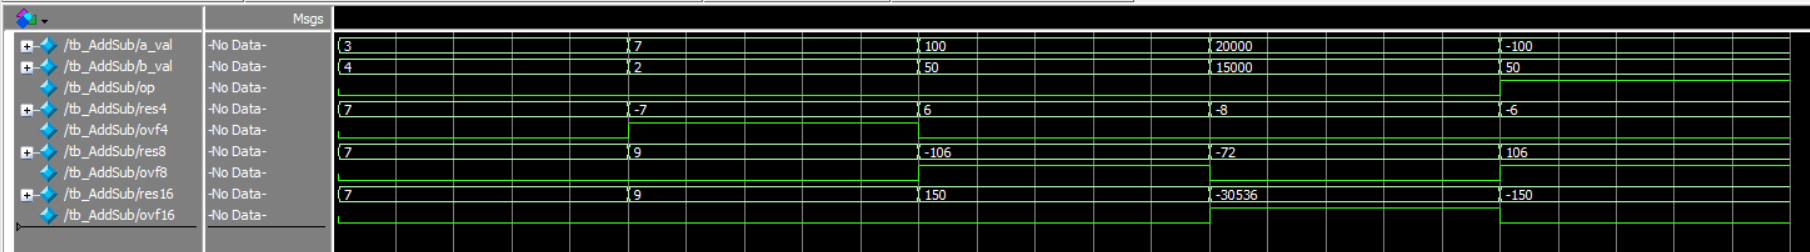
\includegraphics[width=\textwidth]{images/tb_addsub_wave.png}
    \caption{شکل‌موج خروجی میزآزمون ماژول جمع و تفریق برای عرض‌های مختلف}
\end{figure}

\section{پیمانه ضرب‌کننده}
این پیمانه عملگر ضرب سیستم است. از آنجا که در عملیات ضرب، عرض بیت خروجی نسبت به عرض بیت ورودی افزایش می‌یابد، خروجی این ماژول دقیقاً دو برابر عرض ورودی تعریف شده است.

\subsection{پیاده‌سازی کد}
\begin{LTR}
\begin{lstlisting}[title={\rl{کد پیمانه ضرب‌کننده}}]
module Mul #(parameter WIDTH = 8) (
    input signed [WIDTH-1:0] a,
    input signed [WIDTH-1:0] b,
    output signed [(2*WIDTH)-1:0] result
);
    assign result = a * b;
endmodule
\end{lstlisting}
\end{LTR}

\textbf{توضیح خط به خط کد:}
\begin{itemize}
    \item \textbf{خطوط ۱ تا ۵:} تعریف عملوندهای ورودی با عرض \lr{WIDTH} و تعریف درگاه خروجی با عرض $2 \times WIDTH$. این افزایش عرض گذرگاه، راهبرد اصلی برای جلوگیری از اعوجاج در ضرب است.
    \item \textbf{خط ۶:} تخصیص پیوسته\LTRfootnote{Continuous Assignment} با استفاده از عملگر `*`. این خط در زمان سنتز به یک بلوک ضرب‌کننده سخت‌افزاری ترکیبی تبدیل می‌شود که تمامی ارزش‌های مکانی تولید شده را در خروجی بسط‌یافته قرار می‌دهد.
\end{itemize}

\subsection{تحلیل پدیده برش و عدم سرریز}
خروجی با عرض کامل نگهداری شده است و از روش قطع کردن\LTRfootnote{Truncation} بیتی برای خروجی استفاده نشده است، در نتیجه ضرب‌کننده نیازی به پرچم سرریز ندارد.
با این حال، در میزآزمون، زمانی که عددی بزرگتر از ظرفیت ورودی ماژول به سیستم تغذیه می‌شود (مثلاً دادن عدد ۱۲۷ به ماژول ۴ بیتی)، به دلیل ساختار سیم‌کشی میزآزمون که صراحتاً نوشته شده \lr{.a(a\_val[3:0])}، تنها ۴ بیت کم‌ارزشِ آن عدد به ماژول داده می‌شود. عدد ۱۲۷ در قالب ۴ بیتِ پایین خود به صورت \lr{1111} (معادل $-1$) دیده می‌شود. بنابراین مدار عملاً در حال ضرب $-1 \times -1$ بوده و پاسخ $1$ را تولید می‌کند. این پدیده خطای ضرب‌کننده نیست، بلکه رفتار طبیعی برش بیت‌ها در ورودی پورت‌ها پیش از ورود به محاسبات است.

\subsection{آزمون مقیاس‌پذیری و شبیه‌سازی}
میزآزمون شامل سه نمونه ۴، ۸ و ۱۶ بیتی است و سه دسته کلی از مقادیر را مطابق کدهای موجود در فایل تست بررسی می‌کند:

\subsubsection{دسته‌ی نخست: مقادیر مثبت کوچک}
تست با مقادیر $a = 3$ و $b = 2$ انجام شده که پاسخ $6$ در تمامی عرض‌ها با موفقیت ثبت می‌شود.

\subsubsection{دسته‌ی دوم: بیشترین مقادیر مرزی مثبت}
ضرب بزرگترین عدد مثبت هر سیستم در خودش:
\begin{itemize}
    \item \textbf{۴ بیتی:} ضرب $7 \times 7 = 49$.
    \item \textbf{۸ بیتی:} ضرب $127 \times 127 = 16129$.
    \item \textbf{۱۶ بیتی:} ضرب $32767 \times 32767 = 1073676289$.
\end{itemize}

\subsubsection{دسته‌ی سوم: بیشترین مقادیر مرزی منفی}
ضرب منفی‌ترین اعداد در خودشان که منجر به اعداد مثبت بسیار بزرگ می‌شود:
\begin{itemize}
    \item \textbf{۴ بیتی:} ضرب $-8 \times -8 = 64$.
    \item \textbf{۸ بیتی:} ضرب $-128 \times -128 = 16384$.
    \item \textbf{۱۶ بیتی:} ضرب $-32768 \times -32768 = 1073741824$.
\end{itemize}
در تمام این حالات خروجی دقیقاً در ظرفیت دوبرابر شده به درستی محاسبه می‌شود.

\begin{figure}[H]
    \centering
    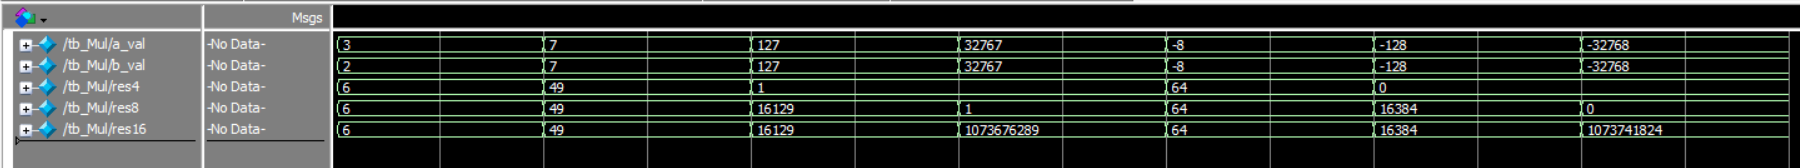
\includegraphics[width=\textwidth]{images/tb_mul_wave.png}
    \caption{شکل‌موج خروجی میزآزمون ماژول ضرب‌کننده}
\end{figure}

\section{پیمانه مزدوج مختلط}
به جای ساخت یک مدار متمم دو مستقل برای قرینه کردن بخش موهومی، این پیمانه نتیجه ضرب بخش موهومی در منفی یک را مستقیماً از ضرب‌کننده مرکزی دریافت کرده و به خروجی هدایت می‌کند تا شرط محدودیت منابع رعایت شود.

\subsection{پیاده‌سازی کد}
\begin{LTR}
\begin{lstlisting}[title={\rl{کد پیمانه مزدوج مختلط}}]
module Conj #(parameter WIDTH = 8) (
    input signed [WIDTH-1:0] A_real,
    input signed [WIDTH-1:0] A_imag,
    input signed [2*WIDTH-1:0] shared_mul_neg_imag,
    output signed [2*WIDTH-1:0] result_real,
    output signed [2*WIDTH-1:0] result_imag,
    output overflow_imag
);
    assign result_real = {{WIDTH{A_real[WIDTH-1]}}, A_real};
    assign result_imag = shared_mul_neg_imag;
    
    // Overflow occurs only when A_imag is the maximum negative value
    assign overflow_imag = (A_imag == {1'b1, {(WIDTH-1){1'b0}}});
endmodule
\end{lstlisting}
\end{LTR}

\textbf{توضیح خط به خط کد:}
\begin{itemize}
    \item \textbf{خط ۹:} بخش حقیقی برای تطابق با سایز مسیر داده، به وسیله عملگرهای تکرار \lr{\{\}} بسط علامت\LTRfootnote{Sign Extension} می‌شود تا ارزش مکانی عدد در فضای دو برابر شده حفظ گردد.
    \item \textbf{خط ۱۰:} قرینه بخش موهومی که پیش‌تر توسط ضرب‌کننده محاسبه شده است، تنها از طریق یک سیم‌کشی مستقیم ترکیبی به درگاه خروجی اختصاص می‌یابد.
    \item \textbf{خط ۱۳:} منطق ترکیبیِ سرریز. در سیستم مکمل دو تنها عددی که قرینه‌اش در همان ظرفیت جا نمی‌شود، منفی‌ترین عدد است (مانند $-128$). این خط بررسی می‌کند که آیا بخش موهومی دقیقاً مساوی با الگوی دودویی\LTRfootnote{Binary} منفی‌ترین عدد (یک ۱ در پرارزش‌ترین بیت و بقیه صفر) است یا خیر.
\end{itemize}

\subsection{تحلیل منطق سرریز}
در سیستم اعداد علامت‌دار، محدوده اعداد نامتقارن است. در صورتی که بخش موهومی عدد ورودی، منفی‌ترین مقدار ممکن در ظرفیت تعیین‌شده باشد، قرینه آن در همان ظرفیت قابل نمایش نخواهد بود. از آنجا که ماژول فرض می‌کند عدد نهایی باید ماهیت \lr{WIDTH} بیتی داشته باشد، با دریافت این مقدار مرزی، سیگنال سرریز را فعال می‌سازد.

\subsection{آزمون مقیاس‌پذیری و شبیه‌سازی}
میزآزمون شامل سه نمونه با عرض‌های ۴، ۸ و ۱۶ بیت است تا عملکرد مدار در قبال حالت‌های مرزی اثبات شود. سیگنال محاسبه قرینه به صورت دستی در میزآزمون تزریق شده است.

\subsubsection{مورد آزمون نخست: مزدوج عادی}
ورودی‌ها: حقیقی $3$ و موهومی $2$. مدار قرینه را به صورت $3 - 2j$ در تمامی نمونه‌ها ثبت کرده و سرریز صفر می‌ماند.

\subsubsection{مورد آزمون دوم: سرریز در نمونه ۴ بیتی}
بخش موهومی ورودی $-8$ داده می‌شود. چون قرینه آن ($+8$) در ۴ بیت جای نمی‌گیرد، ماژول ۴ بیتی پرچم سرریز خود را یک می‌کند.

\subsubsection{مورد آزمون سوم و چهارم: سرریز در نمونه ۸ و ۱۶ بیتی}
با دادن مقادیر $-128$ به نمونه ۸ بیتی و $-32768$ به نمونه ۱۶ بیتی، هر یک از این ماژول‌ها تشخیص می‌دهند که عملوند خارج از حد تقارن است و پرچم خود را فعال می‌کنند.

\begin{figure}[H]
    \centering
    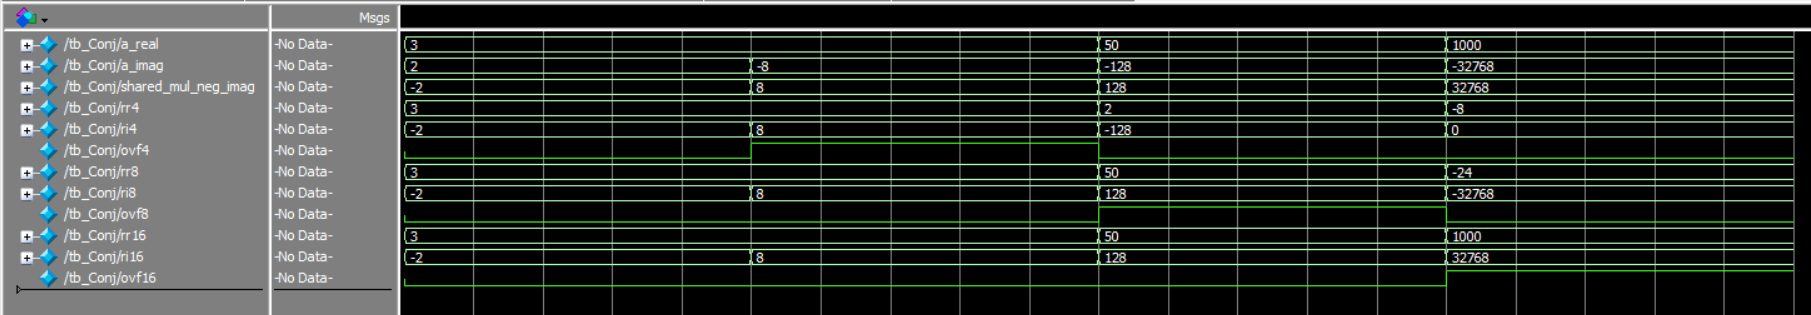
\includegraphics[width=\textwidth]{images/tb_conj_wave.png}
    \caption{شکل‌موج خروجی میزآزمون ماژول مزدوج مختلط}
\end{figure}

\section{پیمانه محاسبه اندازه مربع عدد مختلط}
این پیمانه مقادیر توان دوم و حاصل‌جمع آن‌ها را با اشتراک‌گذاری منابع سخت‌افزاری از ماژول‌های مرکزی دریافت می‌کند.

\subsection{پیاده‌سازی کد}
\begin{LTR}
\begin{lstlisting}[title={\rl{کد پیمانه مجذور اندازه}}]
module Mag2 #(parameter WIDTH = 8) (
    input signed [2*WIDTH-1:0] a2,
    input signed [2*WIDTH-1:0] b2,
    input signed [2*WIDTH-1:0] shared_add_sum,
    output signed [2*WIDTH-1:0] result,
    output overflow
);
    assign result = shared_add_sum;
    // Overflow check: sum of squares is always positive, so MSB should be 0
    assign overflow = shared_add_sum[2*WIDTH-1];
endmodule
\end{lstlisting}
\end{LTR}

\textbf{توضیح خط به خط کد:}
\begin{itemize}
    \item \textbf{خط ۸:} نتیجه نهایی مستقیماً از خروجیِ ماژولِ جمع‌کننده که در مسیر داده قرار دارد کپی می‌شود و هیچ عملیات سخت‌افزاری مضاعفی تولید نمی‌گردد.
    \item \textbf{خط ۱۰:} از آنجا که جمع دو مقدار مربع (توان دوم) قطعاً مقداری مثبت است، هرگاه پرارزش‌ترین بیتِ نتیجه ۱ شود به معنای تغییر علامت ناخواسته ناشی از کمبود ظرفیت (سرریز) است. لذا این خط مستقیماً بیت پرارزش را به درگاه \lr{overflow} اختصاص می‌دهد.
\end{itemize}

\subsection{تحلیل منطق سرریز}
همان‌طور که در کد اشاره شد، تنها شرط سرریز در این ماژول، منفی شدن حاصل‌جمع (به دلیل خروج از ظرفیت مدار) است که از روی ارزش علامت در \lr{shared\_add\_sum} بررسی می‌شود. البته در تست‌بنچ برای اعداد بسیار بزرگ در ماژول ۴ بیتی (مثل 20000)، به علت وراثت و برش بیت‌ها در ورودی پورت، چهار بیت پایین آن مقدار برابر صفر شده و مدار جمع $0+0=0$ را می‌بیند که سرریز ندارد؛ اما برای ۸ و ۱۶ بیت سرریز روشن می‌شود.

\subsection{آزمون مقیاس‌پذیری و شبیه‌سازی}
آزمون‌های مقیاس‌پذیری به شرح زیر بررسی شدند:

\subsubsection{مورد آزمون نخست: مقادیر عادی}
ورودی‌های مربع $4$ و $9$ که مجموع آن‌ها $13$ است. مدار مقدار ۱۳ را بدون خطا خروجی می‌دهد.

\subsubsection{مورد آزمون دوم: سرریز حاصل‌جمع در ۴ بیت}
مقادیر مربع $100$ که مجموع آن‌ها $200$ می‌شود. در نمونه ۴ بیتی که خروجی ۸ بیتی دارد (حداکثر ۱۲۷)، مقدار ۲۰۰ باعث منفی شدن علامت باینری شده و سرریز در مدار ۴ بیتی فعال می‌گردد.

\subsubsection{مورد آزمون سوم: سرریز حاصل‌جمع در ۸ بیت}
مقادیر مربع $20000$ که مجموع آن‌ها $40000$ است. خروجی نهایی سیستم ۸ بیتی دارای ۱۶ بیت عرض است (حداکثر ظرفیت $32767$). مقدار $40000$ باعث سرریز شده و پرچم با موفقیت فعال می‌گردد.

\begin{figure}[H]
    \centering
    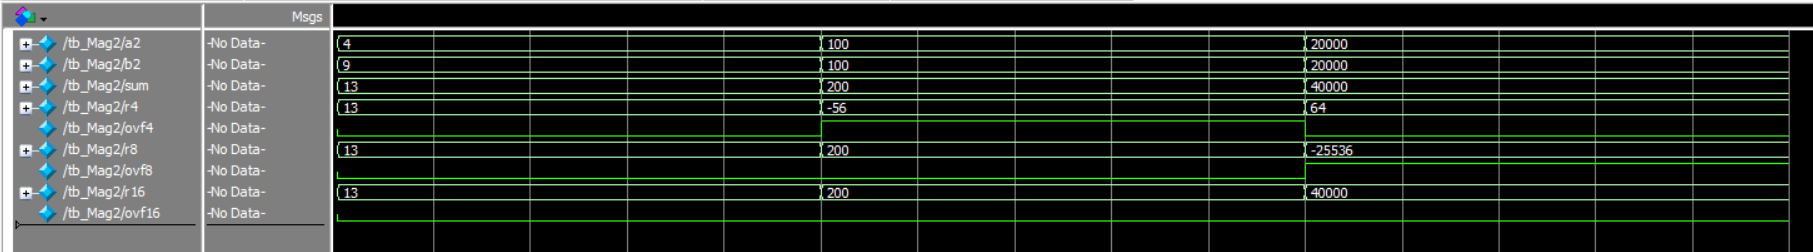
\includegraphics[width=\textwidth]{images/tb_mag2_wave.png}
    \caption{شکل‌موج خروجی میزآزمون ماژول مجذور اندازه}
\end{figure}

\section{پیمانه مسیر داده}
پیمانه مسیر داده، محل استقرار فیزیکی عملگرهاست. این پیمانه با فرمان‌پذیری از واحد کنترل، ورودی‌های مناسب را به سمت تنها ضرب‌کننده و جمع‌کننده موجود در مدار هدایت می‌کند.

\subsection{پیاده‌سازی کد}
\begin{LTR}
\begin{lstlisting}[title={\rl{کد پیمانه مسیر داده}}]
module Datapath #(parameter WIDTH = 8) (
    input clk,
    input rst,
    input [2:0] opcode,
    input signed [WIDTH-1:0] A_real,
    input signed [WIDTH-1:0] A_imag,
    input signed [WIDTH-1:0] B_real,
    input signed [WIDTH-1:0] B_imag,

    input [2:0] sel_mul_1,
    input [2:0] sel_mul_2,
    input [2:0] sel_add_1,
    input [2:0] sel_add_2,
    
    input add_sub_ctrl, 
    
    input en_reg1, en_reg2, en_reg3, en_reg4,
    input en_addout_real, en_addout_imag, en_mulout_real, en_mulout_imag,

    output reg signed [2*WIDTH-1:0] out_real,
    output reg signed [2*WIDTH-1:0] out_imag,
    output zero,
    output overflow,
    output negative_real,
    output negative_imag
);

    wire signed [2*WIDTH-1:0] A_real_ext = {{WIDTH{A_real[WIDTH-1]}}, A_real};
    wire signed [2*WIDTH-1:0] A_imag_ext = {{WIDTH{A_imag[WIDTH-1]}}, A_imag};
    wire signed [2*WIDTH-1:0] B_real_ext = {{WIDTH{B_real[WIDTH-1]}}, B_real};
    wire signed [2*WIDTH-1:0] B_imag_ext = {{WIDTH{B_imag[WIDTH-1]}}, B_imag};

    reg signed [2*WIDTH-1:0] reg1, reg2, reg3, reg4;

    reg signed [WIDTH-1:0] mul_in1, mul_in2;
    always @(*) begin
        case(sel_mul_1)
            3'b000: mul_in1 = A_real;
            3'b001: mul_in1 = A_imag;
            3'b010: mul_in1 = B_real;
            3'b011: mul_in1 = B_imag;
            3'b100: mul_in1 = {WIDTH{1'b1}}; // -1 
            default: mul_in1 = 0;
        endcase

        case(sel_mul_2)
            3'b000: mul_in2 = A_real;
            3'b001: mul_in2 = A_imag;
            3'b010: mul_in2 = B_real;
            3'b011: mul_in2 = B_imag;
            3'b100: mul_in2 = {WIDTH{1'b1}}; // -1 
            default: mul_in2 = 0;
        endcase
    end

    wire signed [2*WIDTH-1:0] mul_out;
    Mul #(.WIDTH(WIDTH)) mult_unit (.a(mul_in1), .b(mul_in2), .result(mul_out));

    reg signed [2*WIDTH-1:0] add_in1, add_in2;
    always @(*) begin
        case(sel_add_1)
            3'b000: add_in1 = A_real_ext;
            3'b001: add_in1 = A_imag_ext;
            3'b010: add_in1 = B_real_ext;
            3'b011: add_in1 = B_imag_ext;
            3'b100: add_in1 = reg1;
            3'b101: add_in1 = reg2;
            3'b110: add_in1 = reg3;
            3'b111: add_in1 = reg4;
            default: add_in1 = 0;
        endcase

        case(sel_add_2)
            3'b000: add_in2 = A_real_ext;
            3'b001: add_in2 = A_imag_ext;
            3'b010: add_in2 = B_real_ext;
            3'b011: add_in2 = B_imag_ext;
            3'b100: add_in2 = reg1;
            3'b101: add_in2 = reg2;
            3'b110: add_in2 = reg3;
            3'b111: add_in2 = reg4;
            default: add_in2 = 0;
        endcase
    end

    wire signed [2*WIDTH-1:0] add_out;
    wire add_overflow;
    AddSub #(.WIDTH(2*WIDTH)) addsub_unit (.a(add_in1), .b(add_in2), .op(add_sub_ctrl), .result(add_out), .overflow(add_overflow));

    wire signed [2*WIDTH-1:0] conj_real, conj_imag;
    wire conj_overflow;
    Conj #(.WIDTH(WIDTH)) conj_unit (.A_real(A_real), .A_imag(A_imag), .shared_mul_neg_imag(mul_out),
                                     .result_real(conj_real), .result_imag(conj_imag), .overflow_imag(conj_overflow));

    wire signed [2*WIDTH-1:0] mag2_result;
    wire mag2_overflow;
    Mag2 #(.WIDTH(WIDTH)) mag2_unit (.a2(reg1), .b2(reg2), .shared_add_sum(add_out),
                                     .result(mag2_result), .overflow(mag2_overflow));

    always @(posedge clk or posedge rst) begin
        if (rst) begin
            reg1 <= 0; reg2 <= 0; reg3 <= 0; reg4 <= 0;
            out_real <= 0; out_imag <= 0;
        end else begin
            if (en_reg1) reg1 <= mul_out;
            if (en_reg2) reg2 <= mul_out;
            if (en_reg3) reg3 <= mul_out;
            if (en_reg4) reg4 <= mul_out;

            if (en_addout_real) begin
                if (opcode == 3'b011) out_real <= conj_real;
                else if (opcode == 3'b100) out_real <= mag2_result;
                else out_real <= add_out;
            end
            else if (en_mulout_real) out_real <= mul_out;

            if (en_addout_imag) out_imag <= add_out;
            else if (en_mulout_imag) begin
                if (opcode == 3'b011) out_imag <= conj_imag;
                else out_imag <= mul_out;
            end
        end
    end

    assign zero = (out_real == 0 && out_imag == 0) ? 1'b1 : 1'b0;
    assign negative_real = out_real[2*WIDTH-1]; 
    assign negative_imag = out_imag[2*WIDTH-1];
    assign overflow = (opcode == 3'b011) ? conj_overflow :
                      (opcode == 3'b100) ? mag2_overflow : add_overflow;

endmodule
\end{lstlisting}
\end{LTR}

\textbf{توضیح خط به خط کد:}
\begin{itemize}
    \item \textbf{خطوط ۳۴ تا ۳۸:} تعریف ثبات‌های چهارگانه برای ذخیره نتایج میانی در عملیات‌های چندچرخه‌ای (مانند ضرب). این ثبات‌ها به عنوان حافظه داخلی مسیر داده عمل می‌کنند.
    \item \textbf{خطوط ۳۷ تا ۶۰:} پیاده‌سازی تسهیم‌کننده‌های\LTRfootnote{Multiplexer} ورودی ضرب‌کننده با استفاده از بلوک ترکیبی \lr{always @(*)}. این مقادیر بر اساس سیگنال‌های انتخابیِ واحد کنترل هدایت می‌شوند.
    \item \textbf{خطوط ۶۳ و ۹۰:} نمونه‌سازی متمرکز و یکتای ضرب‌کننده و جمع‌کننده. این پیاده‌سازی تضمین می‌کند که از نظر سخت‌افزاری تنها یک نمونه از هر کدام سنتز شود.
    \item \textbf{خطوط ۱۰۰ تا ۱۳۰:} بلوک منطق ترتیبی (با تحریک لبه بالارونده ساعت). این بلوک وظیفه ایجاد فلیپ‌فلاپ‌های مورد نیاز برای نگهداری مقادیر ثبات‌ها و خروجی‌های نهایی مدار را بر عهده دارد.
    \item \textbf{خطوط ۱۳۳ تا ۱۳۸:} منطق ترکیبی برای تولید پرچم‌های وضعیت. در اینجا یک تسهیم‌کننده هوشمند بر اساس نوع دستور، سرریز صحیح را به خروجی سیستم هدایت می‌کند.
\end{itemize}

\subsection{تحلیل ساختار مسیر داده}
در این پیمانه دقیقاً یک بار از پیمانه ضرب و یک بار از پیمانه جمع استفاده شده است که تضمین‌کننده رعایت قید طراحی است. همچنین پیمانه‌های مجازی مزدوج و مجذور اندازه با تغذیه از خروجی‌های این دو عملگر، پردازش خود را انجام می‌دهند. بلوک‌های منطق ترتیبی نیز با گرفتن سیگنال فعال‌ساز، نتایج میانی را برای چرخه بعدی در ثبات‌های چهارگانه حفظ می‌کنند.

\section{فرمت دستورها و کدهای عملیاتی}
برای ساده‌سازی طراحی ماشین فرضی، یک ساختار دقیق برای قالب دستور در نظر گرفته شده است. طول هر دستور ۳۵ بیت است تا بتواند عملوندها را به صورت مستقیم در خود جای دهد. ساختار ۳۵ بیتی هر دستور در حافظه به شرح زیر است:
\begin{itemize}
    \item \textbf{بیت‌های ۳۴ تا ۳۲ (۳ بیت):} کد دستور\LTRfootnote{Opcode} که نوع عملیات را مشخص می‌کند.
    \item \textbf{بیت‌های ۳۱ تا ۲۴ (۸ بیت):} بخش حقیقی عملوند اول.
    \item \textbf{بیت‌های ۲۳ تا ۱۶ (۸ بیت):} بخش موهومی عملوند اول.
    \item \textbf{بیت‌های ۱۵ تا ۸ (۸ بیت):} بخش حقیقی عملوند دوم.
    \item \textbf{بیت‌های ۷ تا ۰ (۸ بیت):} بخش موهومی عملوند دوم.
\end{itemize}

جدول زیر مجموعه دستورهای پیشنهادی در این معماری را نشان می‌دهد:
\begin{table}[H]
    \centering
    \begin{tabular}{|c|c|c|}
        \hline
        \textbf{کد دستور} & \textbf{نام دستور} & \textbf{شرح عملیات} \\
        \hline
        \lr{000} & \lr{CADD} & جمع دو عدد مختلط \\
        \hline
        \lr{001} & \lr{CSUB} & تفریق دو عدد مختلط \\
        \hline
        \lr{010} & \lr{CMUL} & ضرب دو عدد مختلط \\
        \hline
        \lr{011} & \lr{CONJ} & محاسبه مزدوج مختلط یک عدد \\
        \hline
        \lr{100} & \lr{CMAG2} & محاسبه اندازه مربع عدد مختلط \\
        \hline
        \lr{101} & \lr{NOP} & بدون عملیات \\
        \hline
    \end{tabular}
    \caption{نقشه کدهای عملیاتی}
\end{table}

دستورهای مزدوج مختلط و اندازه مربع فقط به یک عملوند مختلط نیاز دارند. در این قالب طراحی، عملوند دوم در این دستورها نادیده گرفته شده و تاثیری در خروجی ندارد، لذا با مقدار صفر پر می‌شود.

\section{مدیریت پرچم‌های وضعیت}
در پایان اجرای هر دستور، پرچم‌های وضعیت متناسب با خروجی‌های تولید شده در مسیر داده به‌روزرسانی می‌شوند. این پرچم‌ها به صورت ترکیبی پیاده شده‌اند اما بر اساس قرارداد طراحی، مقادیر آن‌ها تنها در سیکلی که سیگنال معتبر یک می‌شود (پایان دستور) معتبر و قابل استناد است. نحوه مدیریت این پرچم‌ها به شرح زیر است:
\begin{itemize}
    \item \textbf{پرچم صفر:} این پرچم نشان می‌دهد نتیجه نهایی برابر صفر است. برای خروجی مختلط، با استفاده از یک درگاه مقایسه‌گر بررسی می‌شود که آیا هر دو بخش حقیقی و موهومی خروجی دقیقاً برابر با صفر هستند یا خیر.
    \item \textbf{پرچم منفی بودن بخش حقیقی و موهومی:} نشان می‌دهد بخش حقیقی یا موهومی خروجی منفی است. از آنجا که اعداد در نمایش مکمل دو هستند، پرارزش‌ترین بیت هر بخش مستقیماً این وضعیت را نشان می‌دهد.
    \item \textbf{پرچم سرریز:} نشان می‌دهد در نتیجه عملیات جمع، تفریق یا ضرب سرریز رخ داده است. برای مدیریت این وضعیت، یک تسهیم‌کننده هوشمند با بررسی کد دستور فعلی تصمیم می‌گیرد که آیا خطای سرریز را از جمع‌کننده اصلی، از پیمانه مجازی مزدوج و یا از پیمانه مجازی مجذور اندازه به خروجی نهایی منتقل کند.
    \item \textbf{پرچم معتبر:} نشان می‌دهد خروجی عملیات معتبر است و عملیات جاری به پایان رسیده است. این سیگنال در پایان آخرین چرخه اجرای هر دستور، توسط ماشین حالت متناهی فعال می‌گردد.
\end{itemize}

\section{پیمانه واحد کنترل}
واحد کنترل با دریافت کد دستور، عملیات چند چرخه‌ای\LTRfootnote{Multi-Cycle Execution} را با استفاده از یک ماشین حالت متناهی\LTRfootnote{Finite State Machine} مدیریت و کنترل می‌کند.

\subsection{پیاده‌سازی کد}
\begin{LTR}
\begin{lstlisting}[title={\rl{کد پیمانه واحد کنترل}}]
module ControlUnit (
    input clk,
    input rst,
    input start,
    input [2:0] opcode,

    output reg [2:0] sel_mul_1,
    output reg [2:0] sel_mul_2,
    output reg [2:0] sel_add_1,
    output reg [2:0] sel_add_2,
    output reg add_sub_ctrl, // 0 = add, 1 = sub
    output reg en_reg1, en_reg2, en_reg3, en_reg4,
    output reg en_addout_real, en_addout_imag, en_mulout_real, en_mulout_imag,
    output reg valid
);

localparam IDLE    = 5'd0;
localparam CADD1   = 5'd1; localparam CADD2   = 5'd2;
localparam CSUB1   = 5'd3; localparam CSUB2   = 5'd4;
localparam CONJ1   = 5'd5; localparam CONJ2   = 5'd6;
localparam CMUL1   = 5'd7; localparam CMUL2   = 5'd8;
localparam CMUL3   = 5'd9; localparam CMUL4   = 5'd10;
localparam CMUL5   = 5'd11; localparam CMUL6   = 5'd12;
localparam CMUL7   = 5'd13;
localparam CMAG2_1 = 5'd14; localparam CMAG2_2 = 5'd15;
localparam CMAG2_3 = 5'd16; localparam CMAG2_4 = 5'd17;

reg [4:0] state;
reg [4:0] next_state;

always @(*) begin
    next_state = state; 
    case(state)
        IDLE: begin
            if(start) begin
                case(opcode)
                    3'b000: next_state = CADD1;
                    3'b001: next_state = CSUB1;
                    3'b010: next_state = CMUL1;
                    3'b011: next_state = CONJ1;
                    3'b100: next_state = CMAG2_1;
                    default: next_state = IDLE;
                endcase
            end else begin
                next_state = IDLE;
            end
        end
        CADD1:   next_state = CADD2;   CADD2:   next_state = IDLE;
        CSUB1:   next_state = CSUB2;   CSUB2:   next_state = IDLE;
        CONJ1:   next_state = CONJ2;   CONJ2:   next_state = IDLE;
        CMUL1:   next_state = CMUL2;   CMUL2:   next_state = CMUL3;
        CMUL3:   next_state = CMUL4;   CMUL4:   next_state = CMUL5;
        CMUL5:   next_state = CMUL6;   CMUL6:   next_state = CMUL7;
        CMUL7:   next_state = IDLE;
        CMAG2_1: next_state = CMAG2_2; CMAG2_2: next_state = CMAG2_3;
        CMAG2_3: next_state = CMAG2_4; CMAG2_4: next_state = IDLE;
        default: next_state = IDLE;
    endcase
end

always @(posedge clk or posedge rst) begin
    if(rst) state <= IDLE;
    else state <= next_state;
end

always @(*) begin
    sel_mul_1 = 3'b000; sel_mul_2 = 3'b000;
    sel_add_1 = 3'b000; sel_add_2 = 3'b000;
    add_sub_ctrl = 1'b0;
    en_reg1 = 1'b0; en_reg2 = 1'b0; en_reg3 = 1'b0; en_reg4 = 1'b0;
    en_addout_real = 1'b0; en_addout_imag = 1'b0;
    en_mulout_real = 1'b0; en_mulout_imag = 1'b0;
    valid = 1'b0;

    case(state)
        CADD1: begin sel_add_1=3'b000; sel_add_2=3'b010; add_sub_ctrl=1'b0; en_addout_real=1'b1; end
        CADD2: begin sel_add_1=3'b001; sel_add_2=3'b011; add_sub_ctrl=1'b0; en_addout_imag=1'b1; valid=1'b1; end
        CSUB1: begin sel_add_1=3'b000; sel_add_2=3'b010; add_sub_ctrl=1'b1; en_addout_real=1'b1; end
        CSUB2: begin sel_add_1=3'b001; sel_add_2=3'b011; add_sub_ctrl=1'b1; en_addout_imag=1'b1; valid=1'b1; end
        CONJ1: begin sel_add_1=3'b000; sel_add_2=3'b010; add_sub_ctrl=1'b0; en_addout_real=1'b1; end
        CONJ2: begin sel_mul_1=3'b001; sel_mul_2=3'b100; en_mulout_imag=1'b1; valid=1'b1; end
        CMUL1: begin sel_mul_1=3'b000; sel_mul_2=3'b010; en_reg1=1'b1; end
        CMUL2: begin sel_mul_1=3'b001; sel_mul_2=3'b011; en_reg2=1'b1; end
        CMUL3: begin sel_mul_1=3'b000; sel_mul_2=3'b011; en_reg3=1'b1; end
        CMUL4: begin sel_mul_1=3'b001; sel_mul_2=3'b010; en_reg4=1'b1; end
        CMUL5: begin sel_add_1=3'b100; sel_add_2=3'b101; add_sub_ctrl=1'b1; en_addout_real=1'b1; end
        CMUL6: begin sel_add_1=3'b110; sel_add_2=3'b111; add_sub_ctrl=1'b0; en_addout_imag=1'b1; end
        CMUL7: begin valid=1'b1; end
        CMAG2_1: begin sel_mul_1=3'b000; sel_mul_2=3'b000; en_reg1=1'b1; end
        CMAG2_2: begin sel_mul_1=3'b001; sel_mul_2=3'b001; en_reg2=1'b1; end
        CMAG2_3: begin sel_add_1=3'b100; sel_add_2=3'b101; add_sub_ctrl=1'b0; en_addout_real=1'b1; end
        CMAG2_4: begin sel_add_1=3'b100; sel_add_2=3'b100; add_sub_ctrl=1'b1; en_addout_imag=1'b1; valid=1'b1; end
    endcase
end
endmodule
\end{lstlisting}
\end{LTR}

\textbf{توضیح خط به خط کد:}
\begin{itemize}
    \item \textbf{خطوط ۱۷ تا ۲۷:} تخصیص پارامترهای ثابت برای کدگذاری حالاتِ ماشین وضعیت. این روش خوانایی کد را به شدت بالا می‌برد.
    \item \textbf{خطوط ۳۲ تا ۵۸:} بلوک ترکیبی برای تعیین حالت بعدی\LTRfootnote{Next State Logic}. این بخش با بررسی کد دستور، تصمیم می‌گیرد که ماشین از حالت استراحت به کدام زیرشاخه هدایت شود و ترتیب پرش‌ها را تا اتمام دستور مشخص می‌کند.
    \item \textbf{خطوط ۶۰ تا ۶۳:} بلوک منطق ترتیبی (همگام با ساعت) که وضعیت فعلی سیستم را به روزرسانی می‌کند و یا آن را بازنشانی می‌نماید.
    \item \textbf{خطوط ۶۵ تا ۹۶:} بلوک تولید خروجی‌های ترکیبی\LTRfootnote{Output Logic}. در این بخش بسته به حالتِ فعلیِ ماشین، سیگنال‌های کنترلی مسیر داده (نظیر فعال‌سازهای ثبات‌ها و مسیرهای تسهیم‌کننده) یک می‌شوند و در آخرین فاز، سیگنال پایان عملیات نیز فعال می‌گردد.
\end{itemize}

\subsection{زمان‌بندی و مراحل اجرای دستورات چندچرخه‌ای}
اجرای عملیات پیچیده مستلزم اشتراک‌گذاری منابع سخت‌افزاری\LTRfootnote{Resource Sharing} است. جداول زیر سیگنال‌های کنترلی مسیر داده و عملیات ریاضی در هر چرخه را کالبدشکافی می‌کنند.

\subsubsection{دستور جمع دو عدد مختلط}
\begin{table}[H]
    \centering
    \begin{adjustbox}{max width=\textwidth}
    \begin{tabular}{|c|c|c|c|}
        \hline
        \textbf{چرخه} & \textbf{عملیات ریاضی} & \textbf{عملیات در مسیر داده} & \textbf{سیگنال‌های فعال} \\
        \hline
        ۱ & $a + c$ & محاسبه بخش حقیقی & \lr{sel\_add\_1=000, sel\_add\_2=010, en\_addout\_real=1} \\
        \hline
        ۲ & $b + d$ & محاسبه بخش موهومی & \lr{sel\_add\_1=001, sel\_add\_2=011, en\_addout\_imag=1, valid=1} \\
        \hline
    \end{tabular}
    \end{adjustbox}
\end{table}

\subsubsection{دستور تفریق دو عدد مختلط}
\begin{table}[H]
    \centering
    \begin{adjustbox}{max width=\textwidth}
    \begin{tabular}{|c|c|c|c|}
        \hline
        \textbf{چرخه} & \textbf{عملیات ریاضی} & \textbf{عملیات در مسیر داده} & \textbf{سیگنال‌های فعال} \\
        \hline
        ۱ & $a - c$ & محاسبه بخش حقیقی & \lr{sel\_add\_1=000, sel\_add\_2=010, add\_sub\_ctrl=1, en\_addout\_real=1} \\
        \hline
        ۲ & $b - d$ & محاسبه بخش موهومی & \lr{sel\_add\_1=001, sel\_add\_2=011, add\_sub\_ctrl=1, en\_addout\_imag=1, valid=1} \\
        \hline
    \end{tabular}
    \end{adjustbox}
\end{table}

\subsubsection{دستور محاسبه مزدوج مختلط یک عدد}
\begin{table}[H]
    \centering
    \begin{adjustbox}{max width=\textwidth}
    \begin{tabular}{|c|c|c|c|}
        \hline
        \textbf{چرخه} & \textbf{عملیات ریاضی} & \textbf{عملیات در مسیر داده} & \textbf{سیگنال‌های فعال} \\
        \hline
        ۱ & $a$ & عبور بخش حقیقی به خروجی & \lr{en\_addout\_real=1} \\
        \hline
        ۲ & $b \times (-1)$ & قرینه‌سازی بخش موهومی & \lr{sel\_mul\_1=001, sel\_mul\_2=100, en\_mulout\_imag=1, valid=1} \\
        \hline
    \end{tabular}
    \end{adjustbox}
\end{table}

\subsubsection{دستور ضرب دو عدد مختلط}
\begin{table}[H]
    \centering
    \begin{adjustbox}{max width=\textwidth}
    \begin{tabular}{|c|c|c|c|}
        \hline
        \textbf{چرخه} & \textbf{عملیات ریاضی} & \textbf{عملیات در مسیر داده} & \textbf{سیگنال‌های فعال} \\
        \hline
        ۱ & $ac$ & ضرب و ذخیره در ثبات ۱ & \lr{sel\_mul\_1=000, sel\_mul\_2=010, en\_reg1=1} \\
        \hline
        ۲ & $bd$ & ضرب و ذخیره در ثبات ۲ & \lr{sel\_mul\_1=001, sel\_mul\_2=011, en\_reg2=1} \\
        \hline
        ۳ & $ad$ & ضرب و ذخیره در ثبات ۳ & \lr{sel\_mul\_1=000, sel\_mul\_2=011, en\_reg3=1} \\
        \hline
        ۴ & $bc$ & ضرب و ذخیره در ثبات ۴ & \lr{sel\_mul\_1=001, sel\_mul\_2=010, en\_reg4=1} \\
        \hline
        ۵ & $ac - bd$ & تفریق برای بخش حقیقی خروجی & \lr{sel\_add\_1=100, sel\_add\_2=101, add\_sub\_ctrl=1, en\_addout\_real=1} \\
        \hline
        ۶ & $ad + bc$ & جمع برای بخش موهومی خروجی & \lr{sel\_add\_1=110, sel\_add\_2=111, add\_sub\_ctrl=0, en\_addout\_imag=1} \\
        \hline
        ۷ & - & تولید خروجی نهایی & \lr{valid=1} \\
        \hline
    \end{tabular}
    \end{adjustbox}
\end{table}

\subsubsection{دستور محاسبه اندازه مربع عدد مختلط}
\begin{table}[H]
    \centering
    \begin{adjustbox}{max width=\textwidth}
    \begin{tabular}{|c|c|c|c|}
        \hline
        \textbf{چرخه} & \textbf{عملیات ریاضی} & \textbf{عملیات در مسیر داده} & \textbf{سیگنال‌های فعال} \\
        \hline
        ۱ & $a^2$ & محاسبه و ذخیره در ثبات ۱ & \lr{sel\_mul\_1=000, sel\_mul\_2=000, en\_reg1=1} \\
        \hline
        ۲ & $b^2$ & محاسبه و ذخیره در ثبات ۲ & \lr{sel\_mul\_1=001, sel\_mul\_2=001, en\_reg2=1} \\
        \hline
        ۳ & $a^2 + b^2$ & محاسبه مجموع برای بخش حقیقی & \lr{sel\_add\_1=100, sel\_add\_2=101, add\_sub\_ctrl=0, en\_addout\_real=1} \\
        \hline
        ۴ & $0$ & صفر کردن بخش موهومی و خروجی نهایی & \lr{sel\_add\_1=100, sel\_add\_2=100, add\_sub\_ctrl=1, en\_addout\_imag=1, valid=1} \\
        \hline
    \end{tabular}
    \end{adjustbox}
\end{table}

\section{آزمون نهایی سیستم}
یک واحد خط لوله\LTRfootnote{Pipeline} طراحی شده است که وظیفه اتصال اجزا و هماهنگی خواندن از یک حافظه ۳۲ کلمه‌ای را بر عهده دارد. طراحی کاملاً هم‌زمان\LTRfootnote{Synchronous} و مبتنی بر ساعت\LTRfootnote{Clock} است.

\subsection{پیاده‌سازی کد میزآزمون نهایی}
برای طراحی نهایی یک میزآزمون جامع نوشته شده است که چند دستور متوالی را در حافظه قرار داده و اجرای صحیح آن‌ها را بررسی می‌کند. این میزآزمون برای اطمینان از مقیاس‌پذیری و صحت عملکرد ماژول نهایی، سه نسخه مجزا از ماشین را با عرض‌های ۴، ۸ و ۱۶ بیتی شبیه‌سازی می‌کند.
\begin{LTR}
\begin{lstlisting}[title={\rl{کد میزآزمون نهایی سیستم}}]
`timescale 1ns / 1ps

module tb;
    parameter CLK_PERIOD = 10;
    reg clk;
    reg rst;

    // 8-bit System Instance
    wire signed [15:0] fr8, fi8;
    wire fz8, fo8, fnr8, fni8, done8;
    Top #(8) uut8 (.clk(clk), .rst(rst), .final_out_real(fr8), .final_out_imag(fi8),
                   .final_zero(fz8), .final_overflow(fo8), .final_neg_real(fnr8), .final_neg_imag(fni8), .done_all(done8));

    // 4-bit System Instance
    wire signed [7:0] fr4, fi4;
    wire fz4, fo4, fnr4, fni4, done4;
    Top #(4) uut4 (.clk(clk), .rst(rst), .final_out_real(fr4), .final_out_imag(fi4),
                   .final_zero(fz4), .final_overflow(fo4), .final_neg_real(fnr4), .final_neg_imag(fni4), .done_all(done4));

    // 16-bit System Instance
    wire signed [31:0] fr16, fi16;
    wire fz16, fo16, fnr16, fni16, done16;
    Top #(16) uut16 (.clk(clk), .rst(rst), .final_out_real(fr16), .final_out_imag(fi16),
                     .final_zero(fz16), .final_overflow(fo16), .final_neg_real(fnr16), .final_neg_imag(fni16), .done_all(done16));

    initial begin
        clk = 0;
        forever #(CLK_PERIOD/2) clk = ~clk;
    end

    initial begin
        // Allow $readmemh to initialize uut8 naturally
        #1;
        
        // Manual override for 4-bit memory (Add: 2+3j + 1+1j)
        uut4.memory[0] = {3'b000, 4'sd2, 4'sd3, 4'sd1, 4'sd1};
        uut4.memory[1] = {3'b101, 16'd0}; // NOP

        // Manual override for 16-bit memory (Add: 1000+2000j + 500+100j)
        uut16.memory[0] = {3'b000, 16'sd1000, 16'sd2000, 16'sd500, 16'sd100};
        uut16.memory[1] = {3'b101, 64'd0}; // NOP

        // Initiate computation
        rst = 1;
        #(CLK_PERIOD * 2);
        rst = 0;

        // Wait for all scaling tests to finish
        wait (done8 == 1'b1 && done4 == 1'b1 && done16 == 1'b1);
        
        #(CLK_PERIOD * 5);
        $display("===========================================");
        $display("All test cases across 4-bit, 8-bit, and 16-bit executed successfully!");
        $display("===========================================");
        $stop;
    end
endmodule
\end{lstlisting}
\end{LTR}

\textbf{توضیح خط به خط کد:}
\begin{itemize}
    \item \textbf{خطوط ۸ تا ۲۴:} نمونه‌سازی هم‌زمان ۳ ماشین کامپیوتر کاملاً مجزا با عرض‌های ۸، ۴ و ۱۶ بیت جهت انجام تست جامع مقیاس‌پذیری سخت‌افزار.
    \item \textbf{خط ۳۵ تا ۳۹:} بازنویسی دستی\LTRfootnote{Override} فضای حافظه در ماژول‌های ۴ و ۱۶ بیتی جهت تزریق دستورات آزمایشی، بدون ایجاد اختلال در خواندن فایل اصلی حافظه برای سیستم ۸ بیتی.
    \item \textbf{خطوط ۴۹ تا ۵۴:} ایجاد شرط توقف هوشمند با استفاده از عملگر \lr{wait} برای اطمینان از اتمام موفقیت‌آمیز محاسبات در هر ۳ ماشین پیش از چاپ پیام نهایی در کنسول و متوقف ساختن شبیه‌سازی.
\end{itemize}

\subsection{تحلیل موارد آزمون (محتوای حافظه)}
۹ دستور مختلف در حافظه نسخه پایه (۸ بیتی) از طریق فایل متن به فرمت هگزادسیمال مقداردهی شده‌اند. در ادامه روند اجرای این دستورات تحلیل شده است:

\subsubsection{دستور اول: جمع دو عدد مختلط مثبت}
ساختار دستور ۳۵ بیتی: \lr{000\_00000010\_00000011\_00000100\_00000001}
\begin{itemize}
    \item \textbf{کد عملیات:} \lr{000} (جمع)
    \item \textbf{عملوند اول:} \lr{A = 2 + 3j}
    \item \textbf{عملوند دوم:} \lr{B = 4 + 1j}
\end{itemize}
\textbf{شرح عملیات:} $(2+3j) + (4+1j) = 6+4j$. در این حالت، انتظار می‌رود که پس از ۲ چرخه، خروجی برابر با مجموع دو عدد شود و هیچ پرچم خطایی روشن نگردد.

\subsubsection{دستور دوم: جمع دو عدد مختلط منفی}
ساختار دستور ۳۵ بیتی: \lr{000\_11111011\_11111110\_11111111\_11111101}
\begin{itemize}
    \item \textbf{کد عملیات:} \lr{000} (جمع)
    \item \textbf{عملوند اول:} \lr{A = -5 - 2j} (مقادیر \lr{FB} و \lr{FE} در هگزادسیمال)
    \item \textbf{عملوند دوم:} \lr{B = -1 - 3j} (مقادیر \lr{FF} و \lr{FD} در هگزادسیمال)
\end{itemize}
\textbf{شرح عملیات:} $(-5-2j) + (-1-3j) = -6-5j$. پس از ۲ چرخه، پاسخ صحیح در خروجی ظاهر می‌شود و پرچم‌های مربوط به منفی بودن فعال می‌گردند.

\subsubsection{دستور سوم: تفریق دو عدد مختلط با نتیجه منفی}
ساختار دستور ۳۵ بیتی: \lr{001\_00000011\_00000010\_00001000\_00000101}
\begin{itemize}
    \item \textbf{کد عملیات:} \lr{001} (تفریق)
    \item \textbf{عملوند اول:} \lr{A = 3 + 2j}
    \item \textbf{عملوند دوم:} \lr{B = 8 + 5j}
\end{itemize}
\textbf{شرح عملیات:} $(3+2j) - (8+5j) = -5-3j$. مدار عملیات تفریق را انجام داده و پرچم‌های مربوط به اعداد منفی روشن می‌شوند.

\subsubsection{دستور چهارم: ضرب دو عدد مختلط با مؤلفه‌های مثبت و منفی}
ساختار دستور ۳۵ بیتی: \lr{010\_00000010\_11111101\_11111111\_00000100}
\begin{itemize}
    \item \textbf{کد عملیات:} \lr{010} (ضرب)
    \item \textbf{عملوند اول:} \lr{A = 2 - 3j} (مقدار \lr{FD} برای بخش موهومی)
    \item \textbf{عملوند دوم:} \lr{B = -1 + 4j} (مقدار \lr{FF} برای بخش حقیقی)
\end{itemize}
\textbf{شرح عملیات:} $(2-3j) \times (-1+4j) = 10+11j$. پس از طی شدن ۷ چرخه کامل محاسباتی، خروجی به درستی تولید می‌شود که صحت عملکرد شیفت‌ها و محاسبات متوالی در ماشین حالت را ثابت می‌کند.

\subsubsection{دستور پنجم: محاسبه مزدوج مختلط}
ساختار دستور ۳۵ بیتی: \lr{011\_00000100\_00000111\_00000000\_00000000}
\begin{itemize}
    \item \textbf{کد عملیات:} \lr{011} (مزدوج)
    \item \textbf{عملوند اول:} \lr{A = 4 + 7j}
    \item \textbf{عملوند دوم:} (در این دستور با صفر پر شده است)
\end{itemize}
\textbf{شرح عملیات:} $(4+7j)^* = 4-7j$. مدار بخش حقیقی را حفظ کرده و بخش موهومی را در منفی یک ضرب می‌کند تا حاصل تولید شود.

\subsubsection{دستور ششم: محاسبه اندازه مربع عدد مختلط}
ساختار دستور ۳۵ بیتی: \lr{100\_00000011\_11111100\_00000000\_00000000}
\begin{itemize}
    \item \textbf{کد عملیات:} \lr{100} (اندازه مربع)
    \item \textbf{عملوند اول:} \lr{A = 3 - 4j}
    \item \textbf{عملوند دوم:} (در این دستور با صفر پر شده است)
\end{itemize}
\textbf{شرح عملیات:} $|3-4j|^2 = 3^2 + (-4)^2 = 9 + 16 = 25$. مدار پس از ۴ چرخه، عدد نهایی ۲۵ را برای بخش حقیقی و صفر را برای بخش موهومی گزارش می‌دهد.

\subsubsection{دستور هفتم: بررسی خروجی صفر و فعال شدن پرچم مربوطه}
ساختار دستور ۳۵ بیتی: \lr{001\_00000101\_00000101\_00000101\_00000101}
\begin{itemize}
    \item \textbf{کد عملیات:} \lr{001} (تفریق)
    \item \textbf{عملوند اول:} \lr{A = 5 + 5j}
    \item \textbf{عملوند دوم:} \lr{B = 5 + 5j}
\end{itemize}
\textbf{شرح عملیات:} $(5+5j) - (5+5j) = 0+0j$. تفریق دو عدد یکسان منجر به خروجی مطلق صفر شده و پرچم مربوطه در مدار فعال می‌شود.

\subsubsection{دستور هشتم: بررسی حالت‌های مرزی برای وقوع سرریز}
ساختار دستور ۳۵ بیتی: \lr{000\_01100100\_01100100\_01100100\_01100100}
\begin{itemize}
    \item \textbf{کد عملیات:} \lr{000} (جمع)
    \item \textbf{عملوند اول:} \lr{A = 100 + 100j} (مقدار \lr{64} در هگزادسیمال)
    \item \textbf{عملوند دوم:} \lr{B = 100 + 100j}
\end{itemize}
\textbf{شرح عملیات:} $(100+100j) + (100+100j) = 200+200j$. جمع این بردارها از بیشترین مقدار مثبت قابل نمایش در سیستم هشت بیتی (۱۲۷) عبور می‌کند. این عملیات باعث تغییر علامت نامعتبر شده و پرچم مربوطه یک می‌گردد.

\subsubsection{دستور نهم: بدون عملیات}
ساختار دستور ۳۵ بیتی: \lr{101\_00000000\_00000000\_00000000\_00000000}
\begin{itemize}
    \item \textbf{کد عملیات:} \lr{101} (بدون عملیات)
\end{itemize}
\textbf{شرح عملیات:} این دستور به واحد خط لوله اعلام می‌کند که پایان محتوای مفید حافظه فرا رسیده است.

\subsubsection{آزمون مقیاس‌پذیری (۴ و ۱۶ بیتی)}
جهت اطمینان از مقیاس‌پذیری، دو دستور به طور دستی در حافظه سیستم‌های ۴ و ۱۶ بیتی جای‌گذاری گردید:
\begin{itemize}
    \item \textbf{تست ۴ بیتی:} جمع مقادیر $2+3j$ و $1+1j$. خروجی مورد انتظار $3+4j$ است که در خروجی‌های \lr{fr4} و \lr{fi4} مشاهده می‌شود.
    \item \textbf{تست ۱۶ بیتی:} جمع مقادیر $1000+2000j$ و $500+100j$. خروجی مورد انتظار $1500+2100j$ است که در خروجی‌های \lr{fr16} و \lr{fi16} قرار می‌گیرد.
\end{itemize}

\begin{figure}[H]
    \centering
    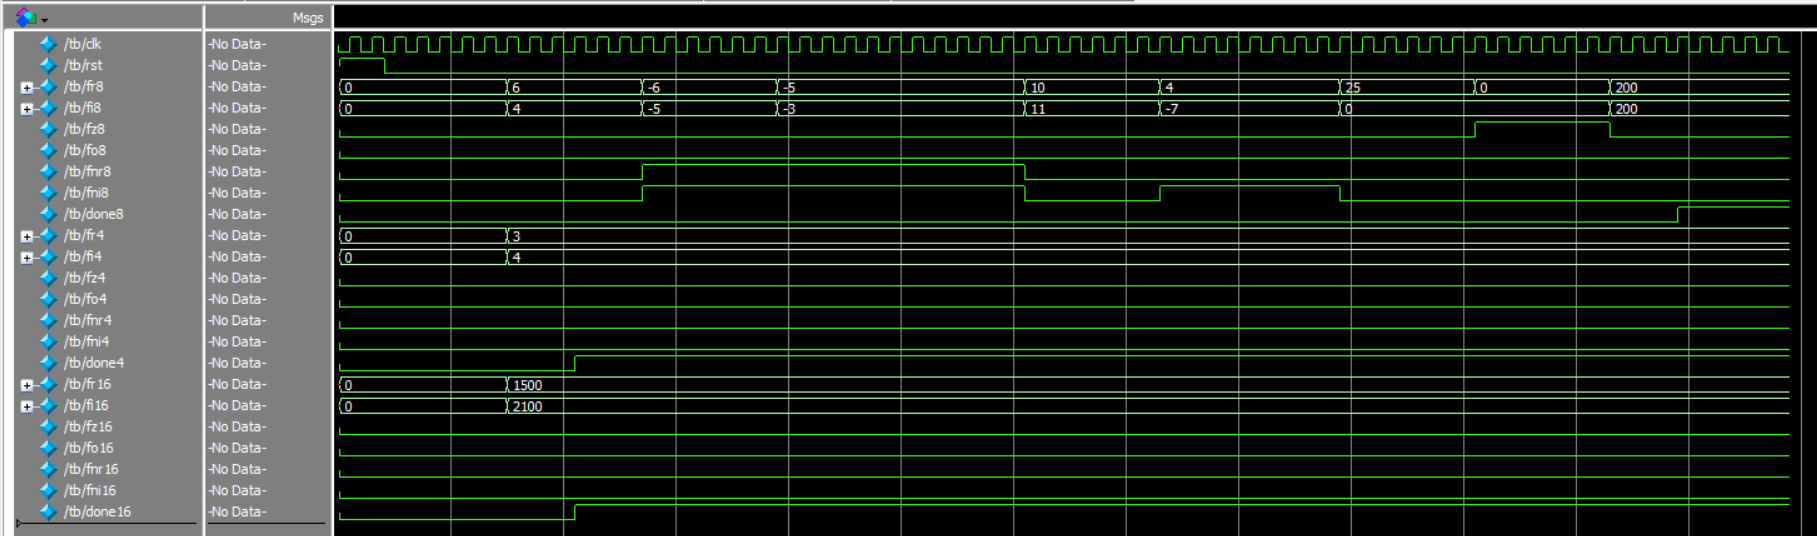
\includegraphics[width=\textwidth]{images/tb_final_wave.png}
    \caption{شکل‌موج خروجی یکپارچه مدار پس از اجرای تمامی دستورات}
\end{figure}

\newpage
\section{بررسی قابلیت سنتز در نرم‌افزار \lr{Quartus}}
یک پروژه در نرم‌افزار \lr{Quartus} ساخته شد و فایل‌های طراحی به آن افزوده شد. نام پیمانه سطح بالا\LTRfootnote{Top-Level Entity} انتخاب شد. برای بررسی اولیه قابل‌سنتز بودن طراحی، مرحله تحلیل و سنتز از مسیر:
\begin{latin}
\begin{verbatim}
Processing > Start > Start Analysis & Synthesis
\end{verbatim}
\end{latin}
اجرا شد. سپس برای تولید نتایج مرحله تطبیق و امکان مشاهده نمای پس از جایابی، کامپایل کامل از مسیر:
\begin{latin}
\begin{verbatim}
Processing > Start Compilation
\end{verbatim}
\end{latin}
انجام گرفت.

پس از تکمیل کامپایل، سه نمای اصلی از مسیرهای زیر باز شدند:
\begin{latin}
\begin{verbatim}
Tools > Netlist Viewers > RTL Viewer
Tools > Netlist Viewers > Technology Map Viewer (Post-Mapping)
Tools > Netlist Viewers > Technology Map Viewer (Post-Fitting)
\end{verbatim}
\end{latin}

در ادامه، خروجی موفقیت‌آمیز بودن کامپایل و همچنین نماهای بررسی‌شده به ترتیب آورده شده است. نمای سطح انتقال ثبات در واقع یک فهرست اتصالات\LTRfootnote{Netlist} بصری است و نرم‌افزار \lr{Quartus} با تشکیل سلسله‌مراتب\LTRfootnote{Hierarchy} مدار، پروسه را بدون خطا طی کرده است.

\begin{figure}[H]
    \centering
    
\includegraphics[width=1\textwidth]{images/quartus_compilation.png}
    \caption{گزارش موفقیت‌آمیز بودن کامپایل کامل و فرآیند سنتز در \lr{Quartus}}
\end{figure}

\begin{figure}[H]
    \centering
    
\includegraphics[width=1\textwidth]{images/rtl_viewer.png}
    \caption{نمای سطح انتقال ثبات (\lr{RTL Viewer})}
\end{figure}

\begin{figure}[H]
    \centering
    
\includegraphics[width=1\textwidth]{images/tech_map_post_mapping.png}
    \caption{نمای نگاشت فناوری پس از نگاشت (\lr{Post-Mapping})}
\end{figure}

\begin{figure}[H]
    \centering
    
\includegraphics[width=1\textwidth]{images/tech_map_post_fitting.png}
    \caption{نمای نگاشت فناوری پس از جایابی و تطبیق (\lr{Post-Fitting})}
\end{figure}

\end{document}